\subsection{Proceso automatizado}

El proceso automatizado se basa en la formalización propuesta en \cite{Maldonado09}, la cual para la definición de la sección de arquetipos usa un sistema de tipos sobre una estructura de árbol. El sistema de tipos modela las restricciones estructurales impuestas por los arquetipos sobre el modelo de referencia. La base del sistema de tipos es la lista de multiplicidad restringida (CML por sus siglas en inglés). El CML es un lenguaje de definición que dentro de la definición del tipo especifica la secuencia válida de hijos de un nodo atributo o objeto de un arquetipo.

El proceso automatizado tiene 3 etapas como se muestra en la Figura \ref{fig:solution}: abstracción, sustitución y definición. Las etapas se repite por cada arquetipo openEHR a crearse a partir de cada recurso FHIR.

\begin{figure}[h]
  \centering
  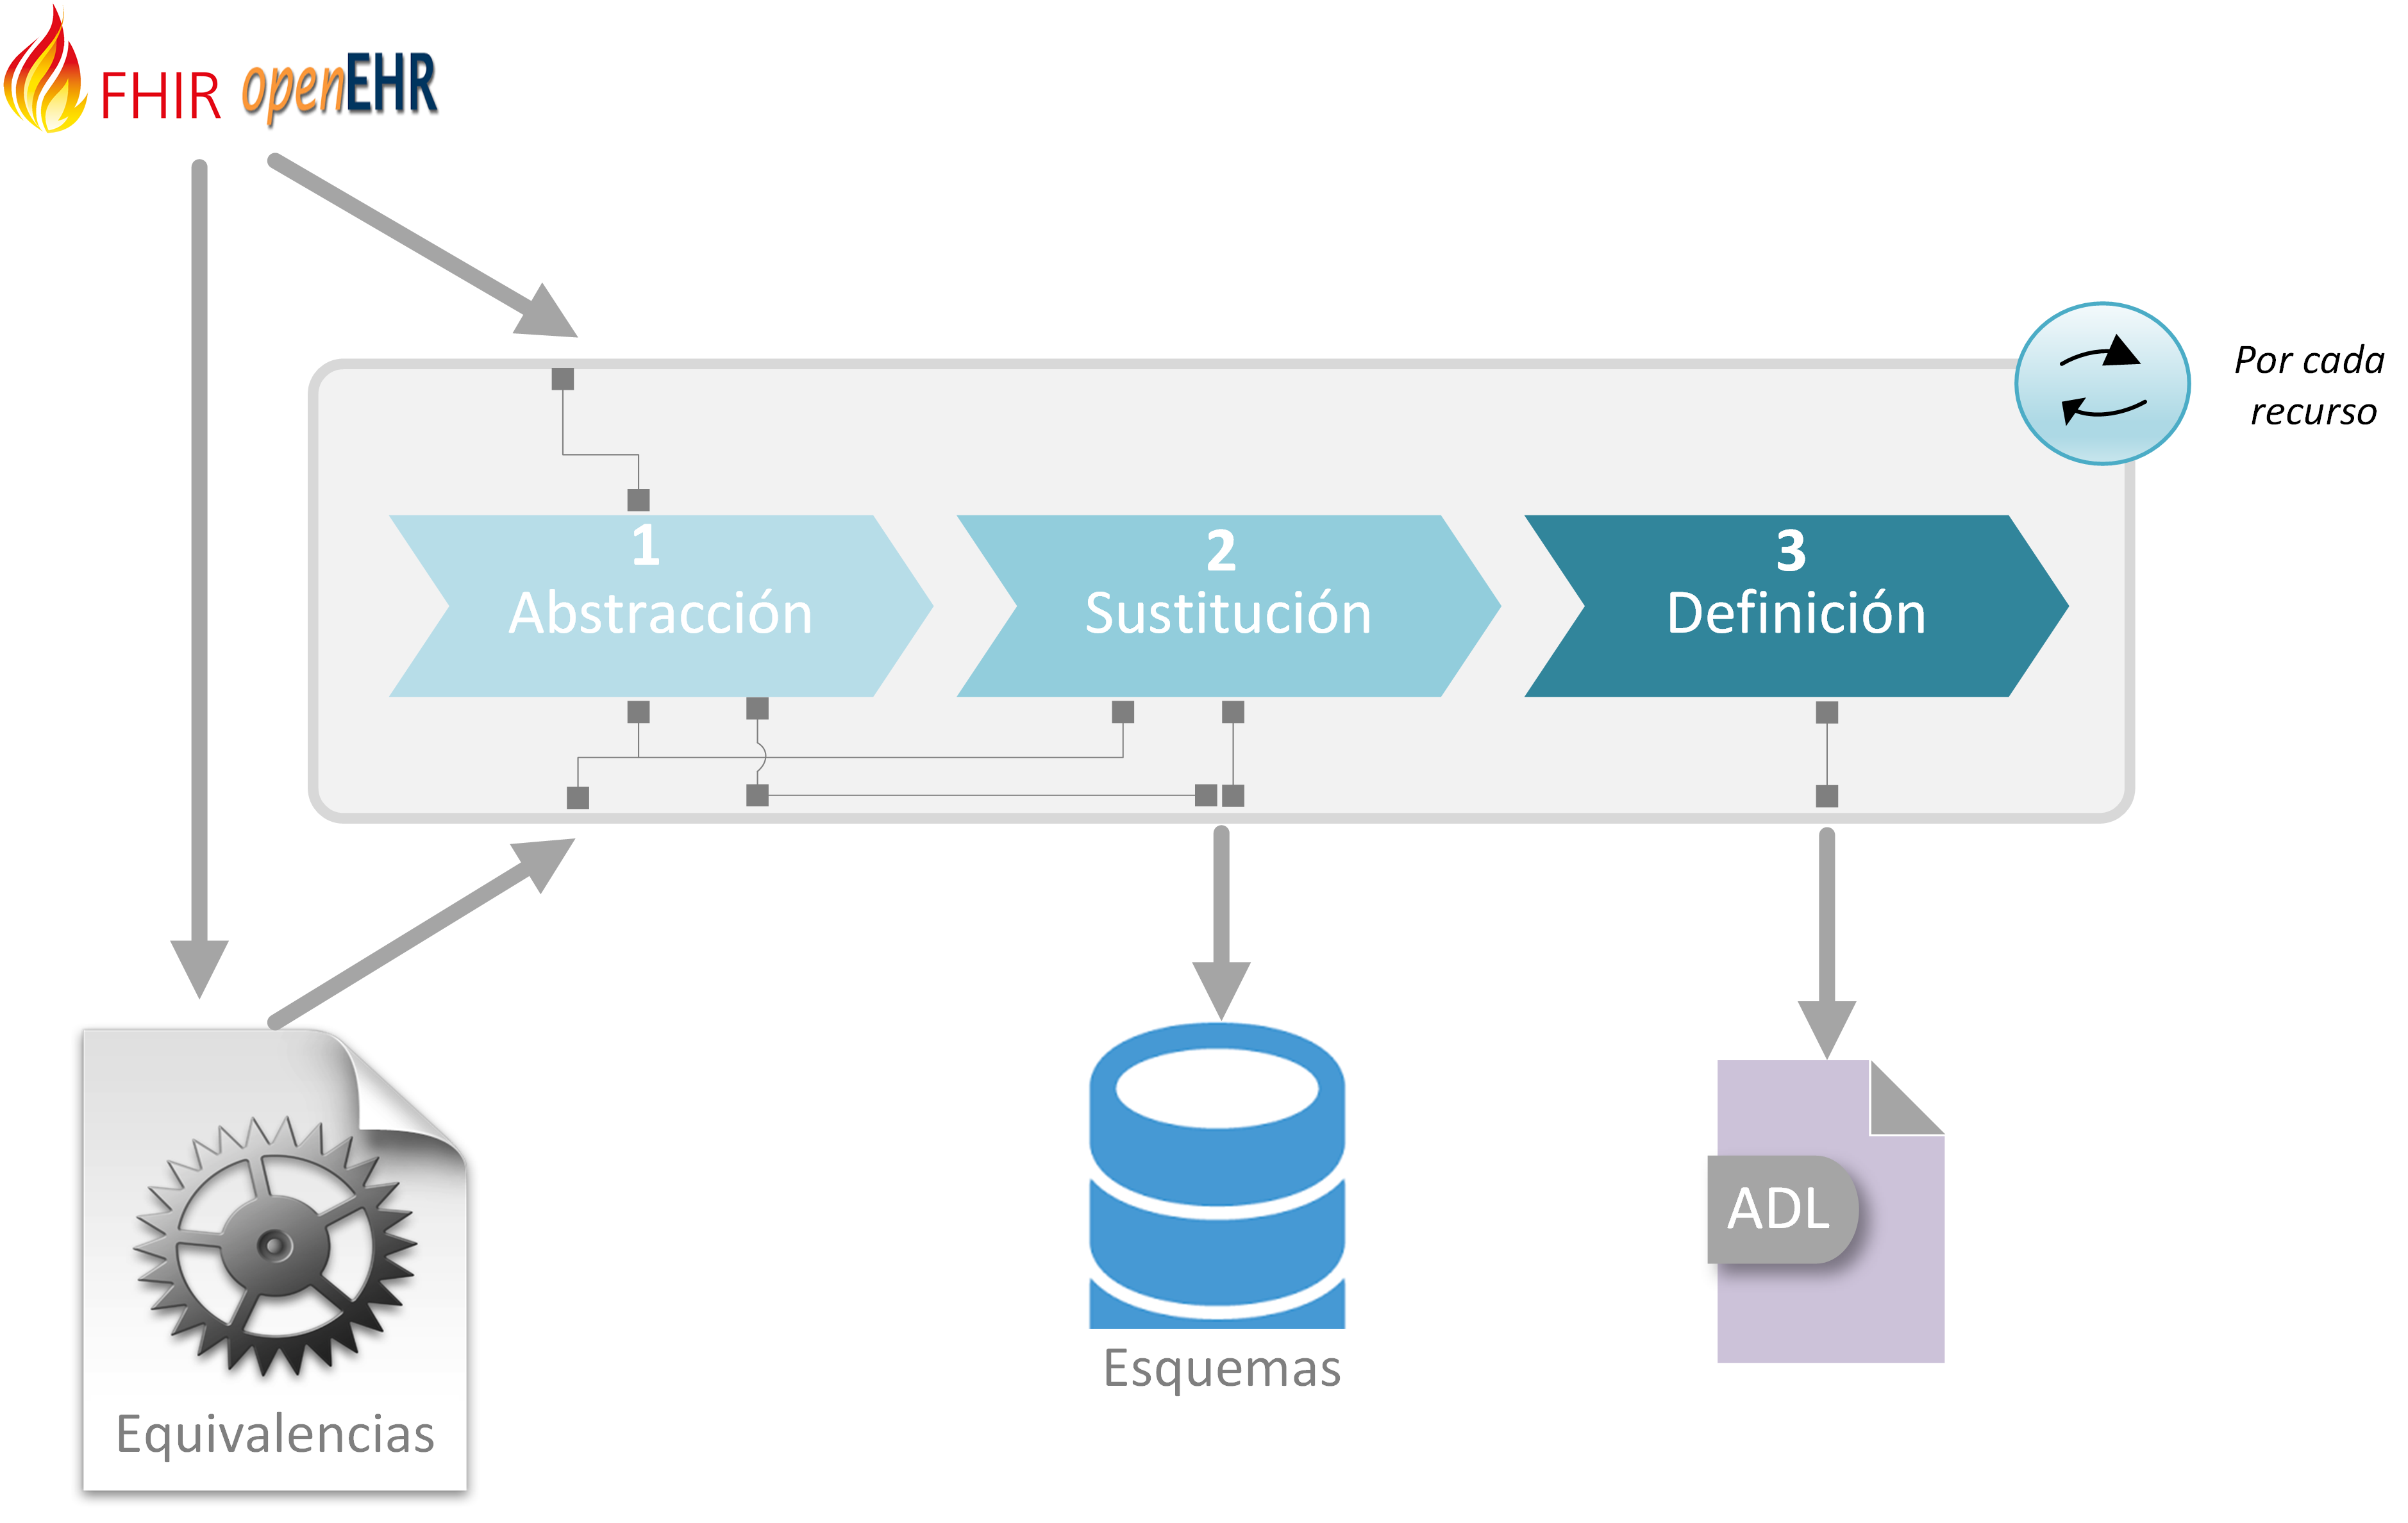
\includegraphics[scale=0.5]{./images/solution}
  \caption{Proceso automatizado.}
  \label{fig:solution}
\end{figure}

\subsubsection{Abstraction stage}

FHIR resource is modeled within a type system similar to the one developed in \cite{Maldonado09}. Each FHIR resource element is abstracted by the type that describes its structure. The definition of a type follows this form:

\begin{align*}
T_t:=p_t\{h_t\}
\end{align*}

\noindent
where \(T_t\) is \(t\)'s name type, \(p_t\) is the predicate that describes the values supported by \(t\) type and \(h_t\) is a CML that specifies child elements that \(t\) type have.

Definition of FHIR resource \(R\) with \(E_1\), \dots , \(E_2\) elements is abstracted with definition type as follows:

\begin{align*}
T_R:=es\_R\{T_{E_1}^{(min_{E_1} \colon max_{E_1})} \dots T_{E_2}^{(min_{E_2} \colon max_{E_2})}\}
\end{align*}

\noindent
where \(T_{E_1}\) is the type that defines \(E_1\) element, \(min_{E_1}\) and \(max_{E_1}\) are the superior and inferior limits of the times \(E_1\) element is allowed to appear in \(R\), respectively. The difference with CML introduced in \cite{Maldonado09} is that in the definition of a type length constraints are not used given they don’t provide additional information to the abstraction of an FHIR resource.

To model bindings, the type system presented in \cite{Maldonado09} is extended, adding binding definitions. A binding definition takes the form:

\begin{align*}
[T_E] := CV
\end{align*}

\noindent
where \(T_E\) is the element type definition to which \(CV\) value set is bound.

For example, when we consider SimplePatient resource (a simplification of FHIR Patient resource \cite{FHIRPatient}) which models a patient who has only one code type gender element \cite{FHIRDataTypes} bound to AdministrativeGender value set \cite{FHIRAdministrativeGender}, it is modeled by the type set::

\begin{align*}
&T_{SimplePatient}:= \\
&\qquad es\_SimplePatient\{T_{SimplePatient.gender}^{(0:1)}\} \\
&T_{SimplePatient.gender}:= \\
&\qquad es\_gender\{T_{SimplePatient.gender.code}^{(1:1)}\} \\
&T_{SimplePatient.gender.code}:= \\
&\qquad es\_code\{\epsilon\} \\
&[T_{SimplePatient.gender.code}] := \\
&\qquad URL \footnotemark[1] \\
\end{align*}

\footnotetext[1]{https://www.hl7.org/fhir/valueset-administrative-gender.html}
A type set that defines an FHIR resource is called an FHIR scheme in this work.


\subsubsection{Etapa de sustitución}

Se transfoma un esquema basado en tipos de datos FHIR generado en la etapa previa en un esquema basado en tipos de datos openEHR. La transformación es directa. Cada definición de un tipo de dato FHIR se reemplaza por una definición de tipo de dato openEHR equivalente. Cada definición de vinculación sobre un tipo de dato FHIR se sustituye por una definición de vinculación sobre un tipo de dato openEHR equivalente. Por ejemplo, el esquema FHIR del recurso SimplePatient se transforma al reemplazar la definición del tipo FHIR code por la definición del tipo openEHR DV\_TEXT equivalente en:

\begin{align*}
&T_{SimplePatient}:= \\
&\qquad es\_SimplePatient\{T_{SimplePatient.gender}^{(0:1)}\} \\
&T_{SimplePatient.gender}:= \\
&\qquad es\_gender\{T_{SimplePatient.gender.DV\_TEXT}^{(1:1)}\} \\
&T_{SimplePatient.gender.DV\_TEXT}:= \\
&\qquad es\_DV\_TEXT\{T_{SimplePatient.gender.DV\_TEXT.value}^{(1:1)}\} \\
&T_{SimplePatient.gender.DV\_TEXT.value}:= \\
&\qquad es\_value\{T_{string}^{(1:1)}\} \\
&[T_{SimplePatient.gender.DV\_TEXT.value}] := \\
& http://hl7.org/ValueSet/administrative-gender \\
&T_{string}:= \\
&\qquad es\_string\{\epsilon\} \\
\end{align*}

A un esquema basado en tipos de datos openEHR se le denomina esquema openEHR en este trabajo. Como se observa, los esquemas FHIR y openEHR de SimplePatient conservan la misma estructura que la definida por el recurso SimplePatient.


\subsubsection{Definition stage}

According to openEHR scheme definitions, an open\-EHR integration archetype is created using Archetype Definition Language (ADL) \cite{openEHRADL}.

An FHIR space name and the name of the FHIR resource the openEHR scheme models are used as an identifier of the new openEHR archetype. For example, the identifier of SimplePatient resource openEHR archetype is:

\begin{lstlisting}
fhir::openEHR-EHR-CLUSTER.SimplePatient.v1.0.0
\end{lstlisting}

For the definition of the new openEHR archetype, open\-EHR scheme types, abstracted from primitive FHIR types, are expressed using ELEMENT structure; and the other openEHR scheme types are expressed using CLUSTER structure. Both structures belong to the openEHR data structure information model \cite{openEHRDataStructures}. For example, SimplePatient resource openEHR archetype definition section uses classes openEHR CLUSTER y openEHR ELEMENT for the \(T_{SimplePatient}\) y \(T_{SimplePatient.gender}\) types, respectively:

\begin{lstlisting}[mathescape=true]
CLUSTER[id1] $\in$ {
  items $\in$ {
    ELEMENT[id2] occurrences $\in$ {0..1} $\in$ {
      value $\in$ {
        DV_TEXT[id3]
      }
    }
  }
}
\end{lstlisting}

Binding definitions are added in the term binding section of the new openEHR archetype. For example, the binding definition of \(T_{SimplePatient.gender.DV\_TEXT.value}\) ty\-pe of SimplePatient resource is transcribed in the term binding section of its equivalent openEHR archetype:

\begin{lstlisting}[escapechar=$]
term_bindings = <
  [``fhir"] = <
    [``id3"] = < URL$\footnotemark$ >
  >
>
\end{lstlisting}

\footnotetext{https://www.hl7.org/fhir/valueset-administrative-gender.html}

OpenEHR archetypes allow the formation of ADL paths, which are used to identify openEHR archetype elements  \cite{openEHRArchitecture}. In this stage, the ADL paths of the new openEHR archetype are created and related to the paths of the elements of their equivalent FHIR resource.

Considering the SimplePatient resource, the relationship established is the following:

\begin{lstlisting}[mathescape=true]
SimplePatient.gender $\Leftrightarrow$ /items[id2]/value[id3]
\end{lstlisting}

